\documentclass[12]{iptex}
\usepackage{underscore}
\usepackage{geometry}
\usepackage{setspace}
\usepackage{titlesec}
\usepackage{titletoc}
\usepackage{tocloft}
\usepackage{booktabs}
\usepackage{adjustbox}
\usepackage{hyperref}
\usepackage{fancyhdr}
\usepackage{lipsum}
\usepackage{romanbar}
\usepackage{etoolbox}
\usepackage{lastpage}
\usepackage{csvsimple}
\usepackage[bottom]{footmisc}
\usepackage{siunitx}
\usepackage{numprint}
\sisetup{round-mode=places, round-precision=0}

% Configurações de Fonte
\renewcommand{\rmdefault}{phv} % Arial
\renewcommand{\sfdefault}{phv} % Arial
\geometry{a4paper, left=2.5cm, right=2cm, top=4.8cm, bottom=3.5cm}
\renewcommand{\baselinestretch}{1.5}

% Configuração do espaçamento antes e depois de títulos
\titlespacing*{\section}{0pt}{1.5\baselineskip}{0.6\baselineskip}
\titlespacing*{\subsection}{0pt}{1.5\baselineskip}{0.6\baselineskip}
\titlespacing*{\subsubsection}{0pt}{1.5\baselineskip}{0.6\baselineskip}
\titlespacing*{\paragraph}{0pt}{1.5\baselineskip}{0.6\baselineskip}
\titlespacing*{\subparagraph}{0pt}{0pt}{0.6\baselineskip}
\titleformat{\section}[hang]{\bfseries\Large}{\thesection}{1em}{} % Ajusta o alinhamento à esquerda

% Configuração de formatação de listas
%\renewcommand{\labelitemi}{\textbullet}
%\pagestyle{fancy}
%\fancyhf{} % Limpa os cabeçalhos e rodapés
%\fancyhead[L]{\vspace*{1.5cm}
\includegraphics[width=4cm]{../figuras/Picture1.png}} % Imagem no cabeçalho
%\fancyfoot[R]{\vspace*{0cm}
\includegraphics[width=8cm]{../figuras/Picture2.png}} % Imagem no rodapé
%\renewcommand{\headrulewidth}{0pt} % Remove a linha horizontal do cabeçalho
%\renewcommand{\footrulewidth}{0pt} % Remove a linha horizontal do rodapé

    \pagestyle{timbrado}




\begin{document}
\thispagestyle{plain} % Aplica o estilo de página customizado à primeira página
\title{\textbf{MONITORAMENTO SISMOLÓGICO} \\
\textbf{RSIS - Rede Sismológica Itá/Machadinho, SC/RS} \\
\textbf{Reservatório de Machadinho, SC/RS} \\
\textbf{BOLETIM SÍSMICO Nº XXXXXX}}
\maketitle

\section{PERÍODO DE ANÁLISE:}

\section{ÚLTIMOS RELATÓRIOS TÉCNICOS:}

\section{ATIVIDADES REALIZADAS:}

\section{RESULTADOS:}

\section{CONSIDERAÇÕES:}

\newpage

\section{COMPLETUDE DOS DADOS}

\begin{figure}[h]
    \centering
    \caption{Gráfico de completude dos dados para o mês de XXX para estação XXX.}
    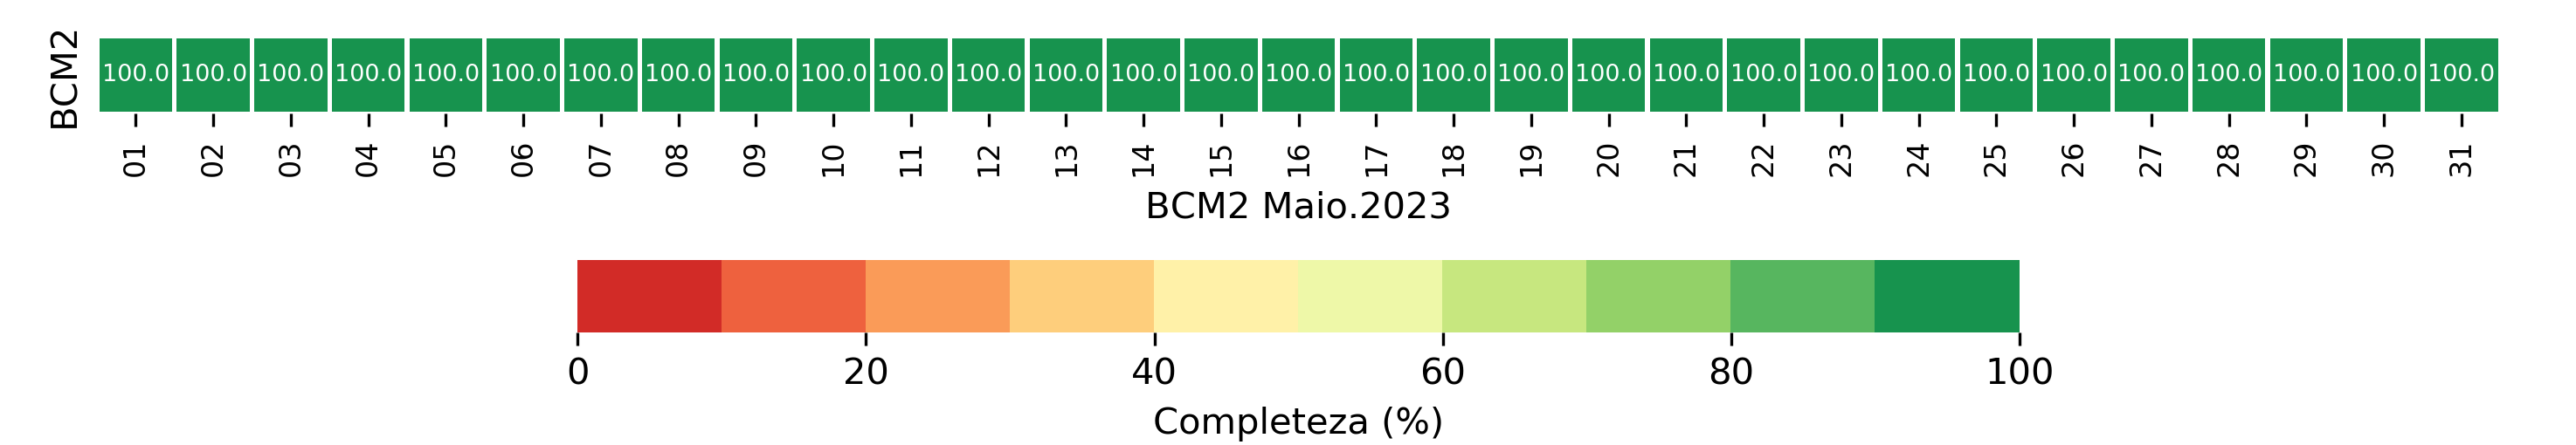
\includegraphics[width=1.0\textwidth]{../figuras/completude.png} % Substitua pelo nome da imagem e ajuste o tamanho
    \caption*{Fonte:IPT}
\end{figure}


\section{TABELA DE EVENTOS}
\begin{center}
\begin{table}[htbp]
    \caption{Dados de Terremotos}
    \label{tab:dados_terremoto}
    \renewcommand{\arraystretch}{1.5} % Ajusta espaçamento entre linhas da tabela
    \small
    \begin{tabular}{ccccccccc} % Defina o número de colunas de acordo com seu arquivo CSV
        \toprule
       \usepackage{underscore}
        ID & Hora de Origem (UTC) & Longitude & Latitude & UTM X & UTM Y & MLv & Energia & Cat \\
        \midrule
         &  & (°) & (°) & (m) & (m) &  & (J) &  \\
        \midrule
        IT_20230630_070654 & 2023-06-30T07:06:54 & -52.1236 & -27.2447 & 388756 & 6985959 & -0.5 & 80.6926 & I \\
        IT_20230623_033615 & 2023-06-23T03:36:15 & -52.0635 & -27.3083 & 394770 & 6978969 & -0.5 & 82.288 & I \\
        IT_20230622_193901 & 2023-06-22T19:39:01 & -52.2639 & -27.2941 & 374921 & 6980353 & -0.6 & 69.5138 & I \\
        IT_20230622_190347 & 2023-06-22T19:03:47 & -52.4587 & -27.6399 & 356096 & 6941839 & 0.9 & 34691.7 & Q \\
        IT_20230621_045910 & 2023-06-21T04:59:10 & -52.3299 & -27.3139 & 368411 & 6978098 & -0.7 & 33.2441 & I \\
        IT_20230619_163424 & 2023-06-19T16:34:24 & -53.0940 & -28.4311 & 294913 & 6853250 & 1.3 & 262839 & Q \\
        gfz2023lsea & 2023-06-16T11:22:00 & -47.4000 & -24.5000 & 256798 & 7288301 & 5.2 & 4.34826e+12 & E \\
        IT_20230613_091716 & 2023-06-13T09:17:16 & -52.3448 & -27.3051 & 366930 & 6979050 & 0.3 & 2568.54 & I \\
        IT_20230611_190546 & 2023-06-11T19:05:46 & -52.1223 & -27.2430 & 388886 & 6986149 & -0.1 & 625.703 & I \\
        IT_20230608_063905 & 2023-06-08T06:39:05 & -52.1233 & -27.2441 & 388790 & 6986031 & -0.6 & 48.8092 & I \\
        IT_20230606_173127 & 2023-06-06T17:31:27 & -52.5289 & -27.4790 & 348949 & 6959577 & 1.2 & 125331 & Q \\
        IT_20230606_003357 & 2023-06-06T00:33:57 & -52.1642 & -27.2142 & 384706 & 6989301 & -0.9 & 17.2632 & I \\
        IT_20230605_203509 & 2023-06-05T20:35:09 & -51.7175 & -27.3387 & 429030 & 6975842 & 0.8 & 29450.1 & Q \\
        IT_20230601_195756 & 2023-06-01T19:57:56 & -52.0606 & -27.2107 & 394964 & 6989781 & 0.9 & 38000.7 & Q \\
        IT_20230601_055456 & 2023-06-01T05:54:56 & -52.1247 & -27.2432 & 388648 & 6986122 & -0.9 & 18.0537 & I \\
        \bottomrule
    \end{tabular}
\end{table}
\end{center}
\newpage

\newpage


\section{MAPA DE EVENTOS}

\begin{figure}[h]
    \centering
    \caption{Mapa de eventos.}
    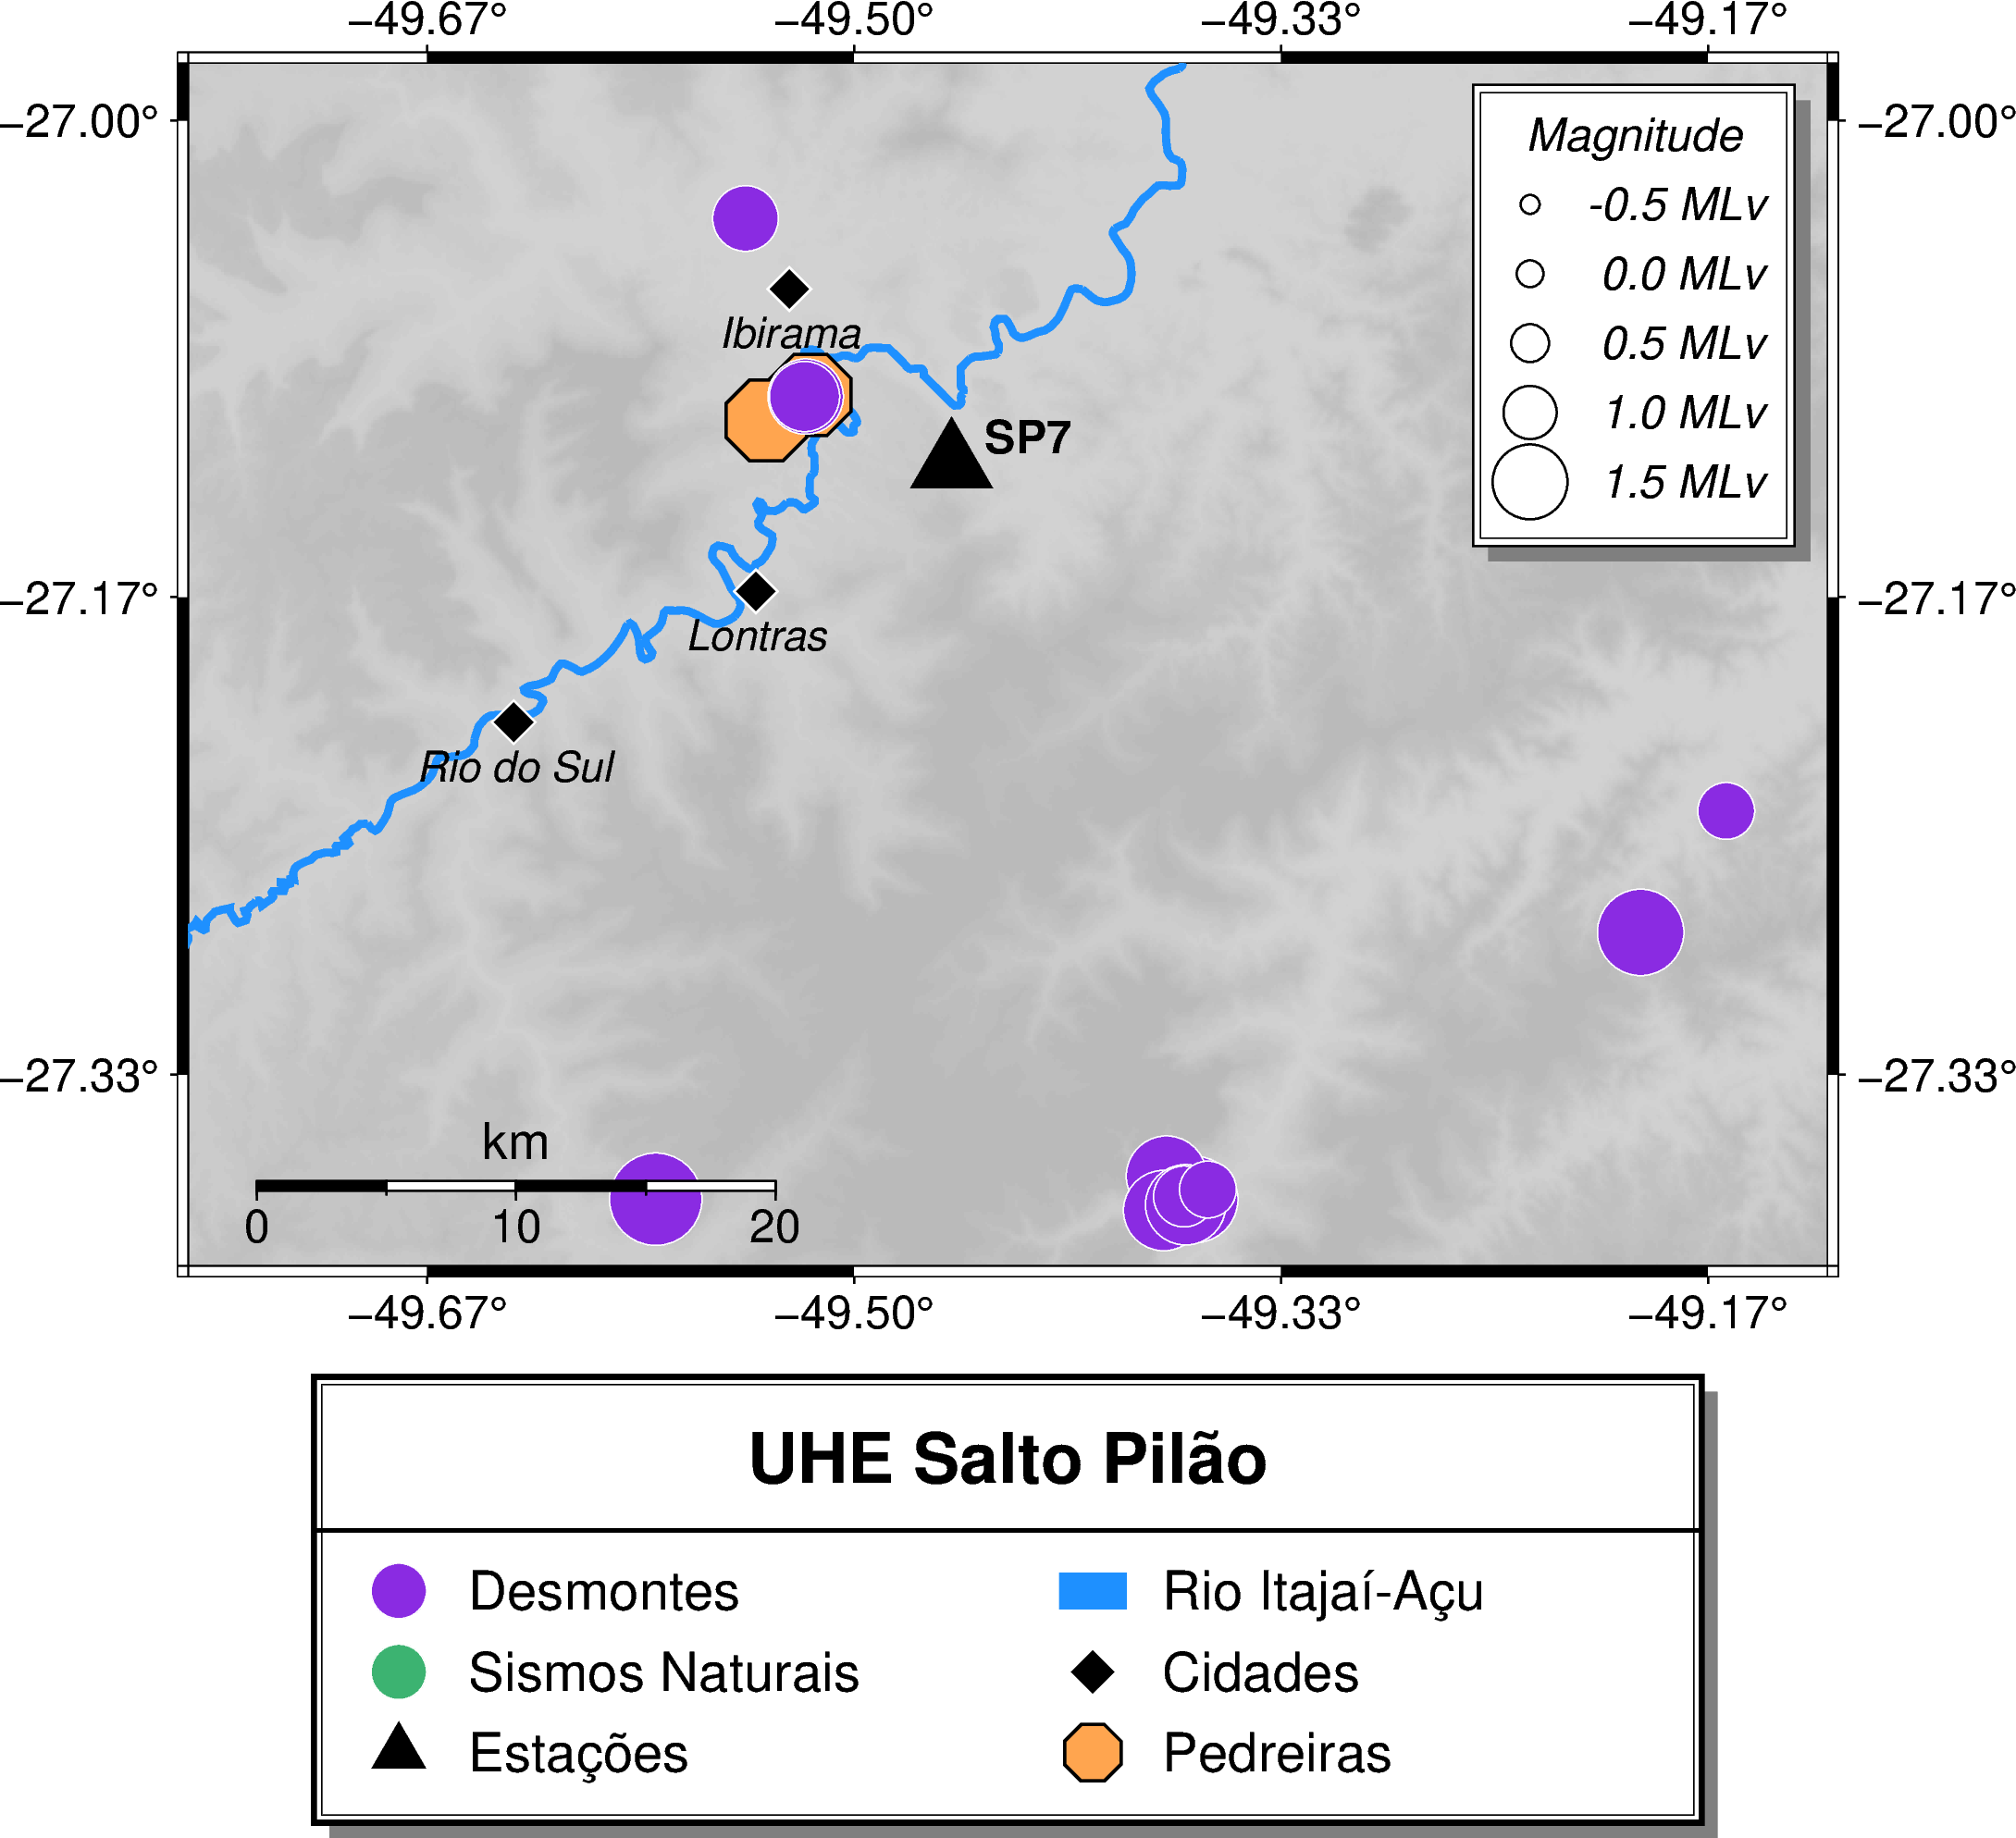
\includegraphics[width=1.0\textwidth]{../figuras/mapaevents.png} % Substitua pelo nome do arquivo de imagem e ajuste o tamanho
    \caption*{Fonte:IPT}
\end{figure}

\newpage

\begin{thebibliography}{9}
  \bibitem{ref1} Autor1. \emph{Título da Referência 1}. Editora, Ano.
  \bibitem{ref2} Autor2. \emph{Título da Referência 2}. Editora, Ano.
  % Adicione suas referências bibliográficas aqui
\end{thebibliography}

\end{document}

